%%%%%%%%%%%%%%%%%%%%%%%%%%%%%%%%%%%%%%%%%%%%%%%%%%%%%%%%%%%%%%%%%%%%%%%%%%
% $Log: warwickthesis.tex,v $
% Revision 1.6  2010/03/11 19:37:41  phrfar
% *** empty log message ***
%
% Revision 1.5  2010/03/10 18:37:49  phrfar
% *** empty log message ***
%
% Revision 1.4  2010/03/10 13:42:09  phrfar
% *** empty log message ***
%
% Revision 1.3  2010/03/09 19:08:04  phrfar
% *** empty log message ***
%
% Revision 1.2  2010/03/08 18:33:41  phrfar
% *** empty log message ***
%
% Revision 1.1.1.1  2010/03/05 17:52:31  phrfar
%
%
%%%%%%%%%%%%%%%%%%%%%%%%%%%%%%%%%%%%%%%%%%%%%%%%%%%%%%%%%%%%%%%%%%%%%%%%%%


%%%%%%%%%%%%%%%%%%%%%%%%%%%%%%%%%%%%%%%%%%%%%%%%%%%%%%%%%%%%%%%%%%%%%%%%%%%%%
% Significant changes were made in 2009, first to work seemlessly with pdflatex
% and secondly to use the setspace package to control linespacing -
% removing some incompatibilities that existed before.
% any comments or problems - contact me  <m.j.hadley@warwick.ac.uk>
%%%%%%%%%%%%%%%%%%%%%%%%%%%%%%%%%%%%%%%%%%%%%%%%%%%%%%%%%%%%%%%%%%%%%%%%%%%%%
%%%
%%% File: utthesis.doc, version 2.0, January 1995
%%% =============================================
%%% Copyright (c) 1995 by Dinesh Das.  All rights reserved.
%%% This file is free and can be modified or distributed as long as
%%% you meet the following conditions:
%%%
%%% (1) This copyright notice is kept intact on all modified copies.
%%% (2) If you modify this file, you MUST NOT use the original file name.
%%%
%%% This file contains a template that can be used with the package
%%% utthesis.sty and LaTeX2e to produce a thesis that meets the requirements
%%% of the Graduate School of The University of Texas at Austin.
%%%
%%% All of the commands defined by utthesis.sty have default values (see
%%% the file
%           warwickthesis.sty
%%%                        for these values).  Thus, theoretically, you
%%% don't need to define values for any of them; you can run this file
%%% through LaTeX2e and produce an acceptable thesis, without any text.
%%% However, you probably want to set at least some of the macros (like
%%% \thesisauthor).  In that case, replace "..." with appropriate values,
%%% and uncomment the line (by removing the leading %'s).
%%%
%%%%%%%%%%%%%%%%%%%%%%%%%%%%%%%%%%%%%%%%%%%%%%%%%%%%%%%%%%%%%%%%%%%%%%%%%%%%%
% all comments starting with %! have been added by M Hadley as
% part of the conversion for the university of warwick
%
%
%\documentclass[11pt,a4paper,twoside]{report}      %% LaTeX2e document.
%%* Removed twoside option
\documentclass[11pt,a4paper]{report}      %% LaTeX2e document.
\usepackage{warwickthesis,setspace,graphicx}     %!  setspace is used to control linepacing
\usepackage{amsmath}
\usepackage{bm}
\usepackage{amssymb}
\usepackage{color}
\usepackage{subfig}
\usepackage{cite}
%\usepackage[numbers]{natbib}
%\usepackage[square]{natbib}                    %! needed for Harvard style of references.
                                                %! for more notes see the bibliography section below

% \mastersthesis                     %% Uncomment one of these; if you don't
 \phdthesis                         %% use either, the default is \phdthesis.

\thesisdraft                       %% Uncomment this if you want a draft
                                     %% version; this will print a timestamp
                                     %% on each page of your thesis.

 \leftchapter                       %% Uncomment one of these if you want
% \centerchapter                     %% left-justified, centered or
% \rightchapter                      %% right-justified chapter headings.
                                     %% Chapter headings includes the
                                     %% Contents, Acknowledgments, Lists
                                     %% of Tables and Figures and the Vita.
                                     %% The default is \centerchapter.
					
%\renewcommand{\familydefault}{cmss}  %! removed April 2009 because the default times font reads more easily
                                     %! for larger blocks of text.%!
                                     %! Added March 2003.
                                     %! This alternative is to use a sans serif font as in
                                     %!  the Warwick Corporate style.
                                     %! The default is Times, which is still acceptable.


% \singlespacing                       %! Uncomment one of these if you want
% \onehalfspacing                   %! single-spacing, space-and-a-half
 \doublespacing                        %! or double-spacing; the default is
                                     %! \oneandhalfspace, which is the
                                     %! minimum spacing accepted by the
                                     %! Graduate School.

\setlength{\textheight}{8.5in}      %! Uncomment this for a slightly
                                     %! longer page. The default is 8in

%! Double sided printing is no longer allowed (March 2008), it caused too many problems at binding,
                              %\setlength{\evensidemargin}{0.15in}  %! Uncomment this line for double sided printing
                                      %! Double-sided printing has recently been
                                      %! allowed by the Graduate School (March 2003)
                                      %! The default is {0.7in} for single sided.
%! Double sided printing is no longer allowed (March 2008), it caused too many problems at binding,

\renewcommand{\thesisdepartmentname}{Department of Physics}    %! The name of
                                                  %   the department

\renewcommand{\thesissubmission}{Submitted to the University of Warwick\\
                                 in partial fulfilment of the requirements\\
                                 for admission to the degree of\\}
%!
%!!!!!!!! default is:
%!
%\renewcommand{\thesissubmission}{Submitted to the University of Warwick\\
%	                        for the degree of Doctor of Philosophy}
%!
%! In the title page this wording will be preceeded by:  thesis\\
%!                 and ended by:  Doctor of Philosophy   (or the
%!                                               selected alternative names
%! use \\ where you want a new line

\renewcommand{\thesisauthor}{Louella Judy Vasquez}    %% Your official name.

\renewcommand{\thesismonth}{July}     %% Your month of graduation.

\renewcommand{\thesisyear}{2010}      %% Your year of graduation.

\renewcommand{\thesistitle}{High Precision Multifractal Analysis in the 3D Anderson Model of Localisation}     %% The title of your thesis; use
                                     %% mixed-case.

%! \renewcommand{\thesistitletypesize}{\LARGE}   %! Put this in if you
                                  %!   want a Large title the default is \large

\renewcommand{\thesisauthorpreviousdegrees}{B.Sc. Physics, M.Sc. Physics}
                                     %% Your previous degrees, abbreviated;
                                     %% separate multiple degrees by commas.

\renewcommand{\thesissupervisor}{Rudolf A. R\"{o}mer	}
                                     %% Your thesis supervisor; use mixed-case
                                     %% and don't use any titles or degrees.


\renewcommand{\thesisauthoraddress}{Department of Physics and Centre for Scientific Computing \\
                                     University of Warwick, Coventry CV47AL, United Kingdom}
                                     %% Your permanent address; use "\\" for
                                     %% linebreaks.
%! For the library declaration page only
 \renewcommand{\thesiscopyrightagree}{agree}
                        %! agreement to allow single photocopies
%! \renewcommand{\thesiscopyrightagree}{do not agree}
                        %! refusal  to allow single photocopies
%! \renewcommand{\thesiscopyrightagree}{agree/do not agree}
                        %! undecided !!
                        %! default is agree


%%%%%%%%%%%%%%%%%%%%%%%%%%%%%%%%%%%%%%%%%%%%%%%%%%%%%%%%%%%%%%%%%%%%%%%%%%%%%
%%%
%%% The following commands are all optional, but useful if your requirements
%%% are different from the default values in utthesis.sty.  To use them,
%%% simply uncomment (remove the leading %) the line(s).

% \renewcommand{\thesisdegree}{...}  %% Uncomment this only if your thesis
                                     %% degree is NOT "DOCTOR OF PHILOSOPHY"
                                     %% for \phdthesis or "MASTER OF ARTS"
                                     %% for \mastersthesis.  Provide the
                                     %% correct FULL OFFICIAL name of
                                     %% the degree.

% \renewcommand{\thesisdegreeabbreviation}{...}
                                     %% Use this if you also use the above
                                     %% command; provide the OFFICIAL
                                     %% abbreviation of your thesis degree.

%\renewcommand{\thesistype}{Thesis}    %% Use this ONLY if your thesis type
                                     %! is NOT "Thesis"
                                     %% Provide the OFFICIAL type of the
                                     %% thesis; use mixed-case.

% \renewcommand{\thesistypist}{...}  %% Use this to specify the name of
                                     %% the thesis typist if it is anything
                                     %% other than "the author".

%%%
%%%%%%%%%%%%%%%%%%%%%%%%%%%%%%%%%%%%%%%%%%%%%%%%%%%%%%%%%%%%%%%%%%%%%%%%%%%%%


%\input header.tex          %! Input declarations, new
                              %theorems etc.


%\graphicspath{{figures/}}
\newcommand{\figwidth}{0.95\columnwidth}
\newcommand{\ud}{\mathrm{d}}
\includeonly{intro_anderson,MFA-theory,MFA-typ,MFA-ens,MFA-partitioning,MFA-PDF,FSS,conclusion}
%\includeonly{intro_anderson,MFA-theory,MFA-typ,MFA-ens,MFA-partitioning,MFA-PDF}

\begin{document}

%%* Made default
\thesiscopyrightpage                 %! Generate the copyright page.

%%* Uncomment a ttitle page.
 %\thesistitlepage                     %% Generate the title page.
\thesistitlecolourpage           %! Generates a COLOUR title page.
%%* Start roman page numbering here for contents, etc
\pagenumbering{roman} %! Begins roman numerals start from page i.
\tableofcontents                     %% Generate table of contents.
\listoftables                      %% Uncomment this to generate listof tables.
\listoffigures                     %% Uncomment this to generate list
                                    %% of figures 


\begin{thesisacknowledgments}        %% Use this to write your
  \input ack.tex                    %% acknowledgments; it can be anything
                                     %% allowed in LaTeX2e par-mode.

                                     %! This following is not needed, but you may like to add it.
%This \lowercase\expandafter{\thesistype} was typeset with
%\LaTeXe\footnote{\LaTeXe{} is an extension of \LaTeX. \LaTeX{} is
%a collection of macros for \TeX. \TeX{} is a trademark of the
%American Mathematical Society. The style package {\em warwickthesis} was
%used.} by \thesistypist.

\end{thesisacknowledgments}

\begin{thesisdeclaration}        %! Use this to declare the extent of
                 %! the original work,
                 %! collaboration, other published
                                 %! material etc.it can be anything
\input declaration.tex

\end{thesisdeclaration}


\begin{thesisabstract}               %% Use this to write your thesis
  \begin{singlespace}       %! uncomment this if you need single spacing
   \input abstract.tex       %!           don't forget the end spacing!
   \end{singlespace}
\end{thesisabstract}

%\begin{thesisabbreviations}       %! Use this to give a list of
                                   %! abbreviateons
                                   %! It can be anything
%\end{thesisabbreviations}         %! allowed in LaTeX2e par-mode.
                                   %!The following may be useful':
                     %!\begin{itemize}
                     %!     \item[symbol]descriptive text..
                     %!\end{itemize}

%\end{thesisabbreviations}
%!!!!!!!!!!!!!!!                     %% Begin your thesis text here; follow
                                     %% the report style and group your text
                                     %% in chapters, sections, etc. eg:
%%* don't need this with one-sided printing
%\newpage{\pagestyle{empty}\cleardoublepage} %! ensure that Chapter 1 starts on an odd
                                           %! page when using double sided printing.
%%* Start arabic numbering of main text here
\pagenumbering{arabic} %! Begins arabic numerals start from page 1.


	
\chapter{Introduction}
\label{chap-INTRO}

%%%%%%%%%%%%%%%%%%%%%%%%%%%%%%%%%%%%%%%%%%%%%%%%%%%%%%%%%%%%%%%%%%%%%%%%%%%%%%%%%%%%%%%%%%%%%%%%%%%%%%%%%%%%%%%%%%%%%%%%%%%%%%%%%%%%%%%%%%%%%%%%%%%%%%%%%%%%%%%%%%%%%%%%%%%%%%%
\section{Anderson Model of Localisation}
\label{sec-AML}

  The interest in this thesis is how electrons behave when the disorder in a lattice is sufficiently strong such that it can cause a transition from a metallic to an insulating state.  By disorder, we mean the presence of impurities and distortions, both being randomly distributed in an otherwise perfect (clean and periodic) lattice.  The picture of disorder for a travelling electron is a sea of random potential.  Localisation of electrons happens as an interference effect due to multiple scatterings of the single particle electronic wavefunction with itself by a random potential.  This phenomenon is first demonstrated by Anderson \cite{And58} in his seminal paper on the absence of diffusion in a simple system of noninteracting particles with random site potential energy and zero external fields.
Since then, the Anderson localisation \cite{KraM93,EveM08} is experimentally observed in microwaves \cite{DalASPM91}, ultrasound \cite{HuSPS08,FaeSPLT09}, light waves \cite{WieBLR97,MooPYB08} quantum waves \cite{HasSMI08,RicRMZ10} and cold atoms \cite{RoaDFF08,BilJZB08}.
%
\begin{figure}
  \centering
  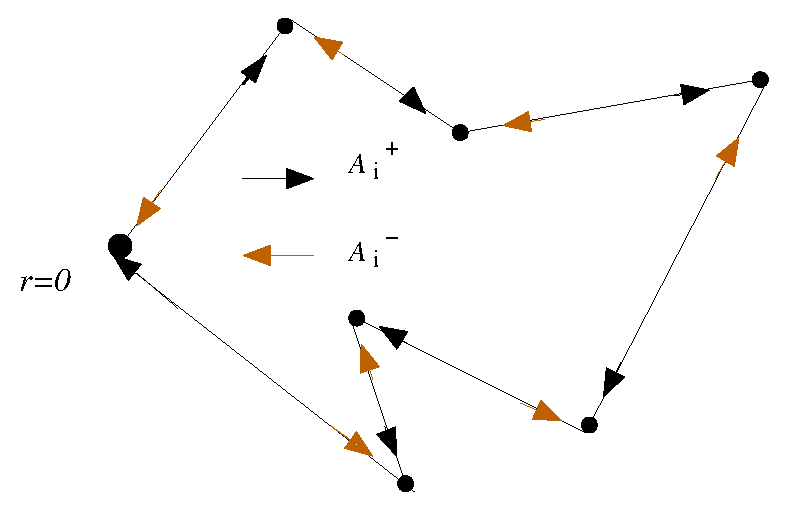
\includegraphics[width=4.5in]{localisation.eps}
   \caption[ A schematic picture of coherent back-scattering of an electron by a random potential.]{  A schematic picture of coherent back-scattering of an electron by a random potential.  An electron returns to its initial position at $r=0$  with probability amplitude $A_i^+(t')$ after a series of scattering events as traced by the black arrows.  The brown arrows trace the corresponding inverse path with probability amplitude $A_i^-(t')$.}
\label{fig-localisation}
\end{figure}
%

If the phase coherence length $l_\varphi$ of the electron is large compared with the system size $L$ then the quantum interference effects become relevant that Anderson localisation for electrons can happen.  This regime is reached when temperature is very low such that inelastic electron-electron and electron-phonon scatterings are suppressed.
%
We can visualize the coherent backscattering that causes localisation in the following manner \cite{Ber83, Ber84}.  We consider an electron at point $\vec{r}=0$ and time $t=0$.  The probability to return to the original point after some time $t=t'$ is given by
%
\begin{equation}
\label{eq-returnPROB}
 \mathcal{P}(t') = \left|\sum_{i\in S}A_i(t')\right|^2,
\end{equation}
%
where $A_i(t')$ is the probability amplitude of an electron that took the $i$th path to return to $\vec{r}=0$ after a number of random scattering events.  The return probability $\mathcal{P}(t')$ is the sum of all possible scattering paths $S$.  Let us consider a simple illustration in Fig.~\ref{fig-localisation}.  For every clockwise path $S_i^+$ traversed by an electron with probability amplitude $A_i^+(t')$, it is true that there exists a corresponding inverse or time reversal path $S_i^-$ with $A_i^-(t')$.  Hence, the set of all scattering paths $S$ is a sum of these two subsets, i.e., $S=S^+ +S^-$.  The return probability of the electron could then be expressed as
%
\begin{eqnarray}
 \mathcal{P}(t')& = & \left|\sum_{i\in S^+}A_i(t') + \sum_{i\in S^-}A_i(t')\right|^2\nonumber\\
                & = & \left|\sum_{i\in S^+} A_i^+(t') + A_i^-(t')\right|^2\nonumber\\
		& = & \sum_{i\in S^+}\left|A_i^+(t') + A_i^-(t')\right|^2 + \sum_{i\neq j \in S^+}\left[A_i^+(t') + A_i^-(t')\right]\times \nonumber\\
		&   & \left[A_j^+(t') + A_j^-(t')\right]^*.
\end{eqnarray}
%
If there is time reversal symmetry such that the phase of the probability amplitude is preserved, i.e., $A_i^+(t')=A_i^-(t')$, then the above equation simplifies into $\mathcal{P}(t')=4\sum_{i\in S^+}\left| A_i(t') \right|^2 $.  In Eq.~\eqref{eq-returnPROB}, the second term accounts for the interference effects between different scattering paths.  In the classical case where the conductivity is defined by the Drude model, this term cancels out due to the destructive interference of the incoherent phases of $A_i(t)$ from the different scattering paths.  The return probability for the classical case reduces to $\mathcal{P}(t')=2\sum_{i\in S^+}\left| A_i(t') \right|^2 $.  The enhancement by a factor of two of the return probability in the presence of coherent multiple backscattering simply means that the electrons are now more spatially restricted in a confined space.  This picture which is brought upon by a significant degree of disorder offers a mechanism for the exponential localisation of the electrons.
%
\begin{figure}
  \includegraphics[width=\figwidth]{extendedVSloc.eps}
   \caption[A comparison between an extended and localised electronic eigenstate.]{ A comparison between an extended and localised electronic eigenstate.  Shown here is the wavefunction amplitude for all $200$ sites of a $1D$ lattice with length $L=200$ in units of lattice spacing and periodic boundary condition imposed.  Using a finite value of the parametrized disorder, the localised and extendend states here are found at the band edge and centre respectively.}
\label{fig-extVSloc}
\end{figure}
%
In Fig.~\ref{fig-extVSloc}, we present the electronic eigenstate for the cases of weak and strong disorder.  In the presence of weak disorder, the wavefunction amplitude $\psi_i$ is on average uniform in space and $\psi \gg 0$ which means that the electron could be found anywhere and hence the state is extended.  On the other hand if the disorder is strong enough to cause large backscatterings that can spatially confined the electron wavefunction then the state is localised.  An example of which is shown in Fig.~\ref{fig-extVSloc} where $\psi_i$ is large in one region and decays in an exponential manner.

%%%%%%%%%%%%%%%%%%%%%%%%%%%%%%%%%%%%%%%%%%%%%%%%%%%%%%%%%%%%%%%%%%%%%%%%%%%%%%%%%%%%%%%%%%%%%%%%%%%%%%%%%%%%%%%%%%%%%%%%%%%%%%%%%%%%%%%%%%%%%%%%%%%%%%%%%%%%%%%%%%%%%%%%%%%%%%%
\section{Scaling Theory of Localisation}
\label{sec-SCALING}

The scaling theory of localisation describes the dependence of the Anderson transition on the dimensionality of the system \cite{AbrALR79,MacK81,MacK83}.  
As a starting point, we consider the size-dependence of the conductance $G$.  The conductance behaves as a measure of the effective disorder.  It is finite for a metallic state and zero for an insulating state.  In units of $e^2/h$ where $e$ and $h$ are the electronic charge and Planck's constant respectively, we have the dimensionless (Thouless) conductance $g=h/e^2~G$.  Here, $g(L,x)$ is only dependent on the system size $L$ and $x$ which represents the set of external parameters such as disorder, Fermi energy, pressure and electron density.  The $g(L,x)$ generally does not depend on the microscopic details (e.g., unit cell) of the material.

The basic assumption of the scaling theory is that given a $d$-dimensional block with volume $(bL)^d$ and integer $b$ its conductance will only be determined by the conductance of the $b^d$ smaller blocks each with volume $L^d$ that build up the larger block.  In other words, the conductance can be expressed as
%
\begin{equation}
\label{eq-scalelawfxn}
 g(bL,x)=\mathcal{F}[g(L,x),b],
\end{equation}
%
which simply means that a rescaling $g(L,x)\rightarrow g(bL,x)$ of the conductance can be defined by the function $g(L,x)$ and scaling factor $b$.  In differential form, Eq.~\eqref{eq-scalelawfxn} is
%
\begin{equation}
\label{eq-scalelawbeta}
 \frac{\ud g(L,x)}{\ud L}=\beta(g).
\end{equation}
%
Equation \eqref{eq-scalelawbeta} states that the scaling function $\beta$ is only dependent on $g(L,x)$.  We will now obtain the assympotic behaviour of $\beta(g)$ for the limiting cases of small (localised insulating state) and big (extended metallic state) $g(L,x)$.  When the random potential is weak, the electronic state is extended and plane wave-like.  For a $d$-dimension system of size $L$, the Ohmic conductance for a metal is $G=1/R=\sigma L^{d-2}$ where $G$ is simply the inverse of the resistance $R$ and $\sigma$ is the d.c. conductivity of the material. 
  When the disorder is sufficiently strong, the states very near the Fermi energy are localised.  Electronic states nearly equal in energy are far apart from each other in space such that hopping between these states does not happen.
The electronic wavefunction is exponentially localised and the conductance assumes the form $g=g_0~\mathrm{e}^{-L/\xi}$.  The localisation length $\xi$ defines the spatial extent of the wavefunction and here $L>>\xi$.  

\begin{figure}
  \centering
  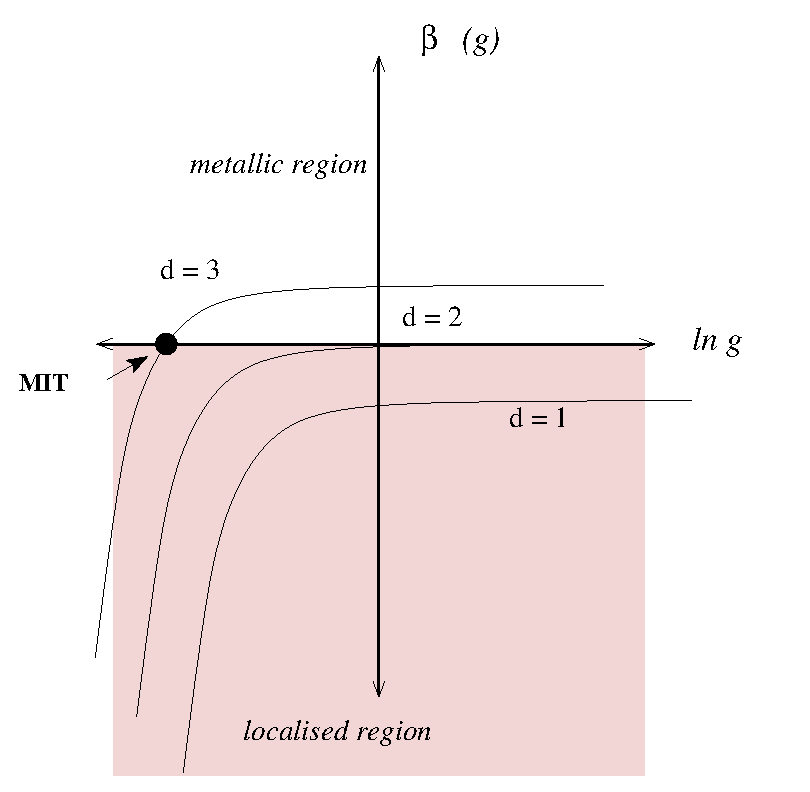
\includegraphics[width=4.0in]{betafxn.eps}
   \caption[ A schematic diagram showing the behaviour of the scaling function $\beta(g)$ for dimensions $d=1,2,3$.]{ A schematic diagram showing the behaviour of the scaling function $\beta(g)$ for dimensions $d=1,2,3$.  The metallic region is $\beta>0$.  The localised region is the shaded part corresponding to $\beta<0$. A crossing point at $\beta=0$ for $d>2$ indicates an MIT.  According to the scale dependence of $\beta(g)$, there are no extended states for $d\leq2$ in the presence of a finite degree of disorder.}
\label{fig-betafxn}
\end{figure}

The scaling theory assumes that $\beta(g)$ is monotonic and that a continuous behaviour connecting the localised and extended regimes is possible.  The scale-dependence of $\beta(g)$ is shown in Fig.~\ref{fig-betafxn}.  When $\beta > 0$ in the metallic case, the conductance increases with $L$ and diverges in the thermodynamic limit.  The asymptotic behaviour of the function is $\beta(g)=d-2$.  For $\beta<0$, $g$ decreases with $L$ and becomes zero as $L\rightarrow\infty$.  In the latter case, $\beta(g)=\ln (g/g_0)$.  The system becomes more metallic or insulating as it gets bigger in $L$.  
For $d\leq2$, $\beta(g)$ is always negative.  This means that in $d\leq2$ unless it is a perfect conductor all electronic wavefunctions will always be localised and the system will always be an insulator in the presence of a finite disorder.
This is not the case for $d=3$.  A crossover at $\beta =0$ between the metallic and insulating regimes exists as seen in Fig.~\ref{fig-betafxn}.  At this critical point, the conductance does not depend on the system size and this scale-invariance implies that exactly at this point there is a metal to insulator transition (MIT).  The set of parameters $x$ such as disorder controls the value of $g(L,x)$.  For instance, if the disorder is weak then the state is in the localised region.  If the disorder is strong enough, it is an extended state.

Near the critical transition, there is only one relevant length scale.  It is the localisation length $\xi$ in the localised regime or the correlation length between wavefunction amplitudes in the extended region.  The localisation (correlation) length diverges near the MIT and since it depends on $x$ then it should diverge at the critical point $x=x_c$ as expressed by \cite{Car87}

%why localisation length diverges
%why is there one relevant length scale

\begin{equation}
 \xi \propto |x-x_c|^{-\nu}.
 \label{eq-XIdef}
\end{equation}
The critical exponent $\nu$ defines the Anderson transition and is the same regardless of the microscopic details for all systems belonging to one universality class or systems sharing the same symmetry in the Hamiltonian.
Furthermore, the scaling theory states that near the critical point of the Anderson transition all systems with finite length $L$ can be scaled by the localisation length for $L\rightarrow \infty$.  If so then the conductance or any measure characterizing critical properties can be described by one scaling function as

\begin{equation}
 g(L,x)=\mathcal{F}\left(\frac{L}{\xi}\right).
 \label{eq-oneparamfxn}
\end{equation}
Equations \eqref{eq-scalelawfxn}, \eqref{eq-scalelawbeta} and \eqref{eq-oneparamfxn} together is also known as one parameter scaling theory \cite{KraM93,MacK81,MacK83}.

%%%%%%%%%%%%%%%%%%%%%%%%%%%%%%%%%%%%%%%%%%%%%%%%%%%%%%%%%%%%%%%%%%%%%%%%%%%%%%%%%%%%%%%%%%%%%%%%%%%%%%%%%%%%%%%%%%%%%%%%%%%%%%%%%%%%%%%%%%%%%%%%%%%%%%%%%%%%%%%%%%%%%%%%%%%%%%%
\section{Numerical Model}
\label{sec-NUMERICS}

To model an electron in a disordered lattice, we use the single-electron tight-binding Anderson Hamiltonian as simply given by
%
\begin{equation}
 \mathcal{H}=\frac{p^2}{2m}+\sum_{i=1}^N U_i(r-R_i),
\end{equation}
%
where $m$ is an effective mass of an electron with momentum $p$, $U_i$ is the potential energy of the $i$-th ion located at $r-R_i$ and the summation is for the total number of ionic sites $N$.
The discrete version of this Hamiltonian in terms of lattice site basis is
%
\begin{equation} \label{anderson_H1} 
\mathcal{H}=\sum_{i} \varepsilon_{i}~\vert i\rangle\langle i\vert + \sum_{i\neq j} t_{ij}~\vert i\rangle\langle j\vert,
\end{equation}
%
for a simple case of only one state per site.
%
Here, $|i\rangle$ is a basis denoting the electronic state localised at position $i=(x,y,z)$ in a cubic lattice of volume $V=L^3$
, $t_{ij}$ are nearest-neighbour hopping amplitudes between sites $i$ and $j$, and $\varepsilon_i$ is the $i$-th site potential energy.  
In this work, we only consider Hamiltonians that fall under the symmetry class of Gaussian orthogonal ensemble, i.e., the $\mathcal{H}$ has time-reversal and spin-rotational symmetries.  The hopping term is set to unity $t=1$ and disorder is introduced into the model by randomising the values of the site potential energies $\varepsilon_i$.
We consider $\varepsilon_i$ to have a uniform probability distribution in the interval $[-W/2,~W/2]$, where $W$ parametrizes the strength of the disorder.  For a critical state at the band centre, $W=W_c\approx16.5$, above the critical disorder $W_c$ all eigenstates are localised \cite{SleMO03,SleMO01,OhtSK99,MilRSU00}.  To minimize boundary effects, periodic boundary conditions are used.
Due to the universality of the Anderson transition, some of the the critical properties such as the critical exponent will not depend on the details of the Hamiltonian.  Hence, a simple tight-binding model for a cubic lattice as just described is able to give the critical properties of the transition.

The $L^3\times L^3$ Hamiltonian matrix has random values in the diagonal elements which represent the site potential energies.  If only nearest neighbor hopping is considered, it is also a sparse matrix with a few off-diagonal elements equal to one.  The matrix is diagonalized using the JADAMILU package \cite{BolN07} which is a Jacobi-Davidson implementation with an integrated solver based on the incomplete-$LU$-factorization package (ILUPACK) \cite{SchBR06, BolN07}.
We have considered eigenstates only in the vicinity of the band centre $E=0$ where the Anderson transition is found when $W_c\approx 16.5$.  We take about five eigenstates in a small energy window around $E=0$ for any given realizations of disorder.

%%%%%%%%%%%%%%%%%%%%%%%%%%%%%%%%%%%%%%%%%%%%%%%%%%%%%%%%%%%%%%%%%%%%%%%%%%%%%%%%%%%%%%%%%%%%%%%%%%%%%%%%%%%%%%%%%%%%%%%%%%%%%%%%%%%%%%%%%%%%%%%%%%%%%%%%%%%%%%%%%%%%%%%%%%%%%%%
\section{Fractal Dimension and Multifractals}
\label{sec-MFABASICS}

%capacity dimension
%Mandelbrot fractal
%characteristic length scale
%Examples of multifractals in nature 

Consider a line segment with unit length $L=1$.  Cover the line with spheres of diameter $l=1/a$.  Other geometrical shapes may be used as well.  The least number of spheres that is needed to fully cover the line segment, $N(l)$, is exactly equal to $(L/l)^{D_f}$ where $D_f$ is called the dimension of the support or simply the dimension of a system.  Extending this to a square and a cube, we can say that $N(l)\propto l^{-D_f}$.  For these three cases of the line segment, square and cube, it is clear to see that $D_f=1,2,3$ respectively.  The value of $D_f$ for the above examples is simply equivalent to the Euclidean or topological dimension.  

Let us now apply the same procedure to a deterministic fractal such as the Mandelbrot-Given fractal as shown in Fig.~\ref{fig-mandelbrot}.  We consider its initial structure which is composed of eight line segments each with length $L=1/3$.  This fractal structure is being generated by replacing each line segment with the initial structure.  For this fractal, $N(l=\frac{1}{3})=8$, that is eight spheres with diameter $l=1/3$ is needed to separately contain each of the eight line segments of the initial structure.  If $l$ is reduced then $N(l=(\frac{1}{3})^2)=8^2$.  Recall that $N(l)\propto l^{-D_f}$, hence $D_f=-\mathrm{\ln}[N(l)]/\mathrm{\ln}[l]$.  For the Mandelbrot-Given fractal, the dimension $D_f$ is a non-integer value of $D_f=\mathrm{\ln}_3 8$ that is less than the Euclidean dimension $d$.  The physical meaning of a non-integer $D_f$ and $D_f<d$ is that the rate at which the volume increases is slower than the increase in linear length $L$.
%
Systems that are defined by one non-integer dimension are called self-similar structures or simply fractals.  Self-similar because they are scale invariant under isotropic scale transformation which means that the volume of the system increases uniformly in every spatial directions. 
Fractals occuring in nature are random fractals.  Their structure could not be exactly formed by repeated generation of a pattern but in a statistical sense they are self similar.
%
\begin{figure}
  \centering
  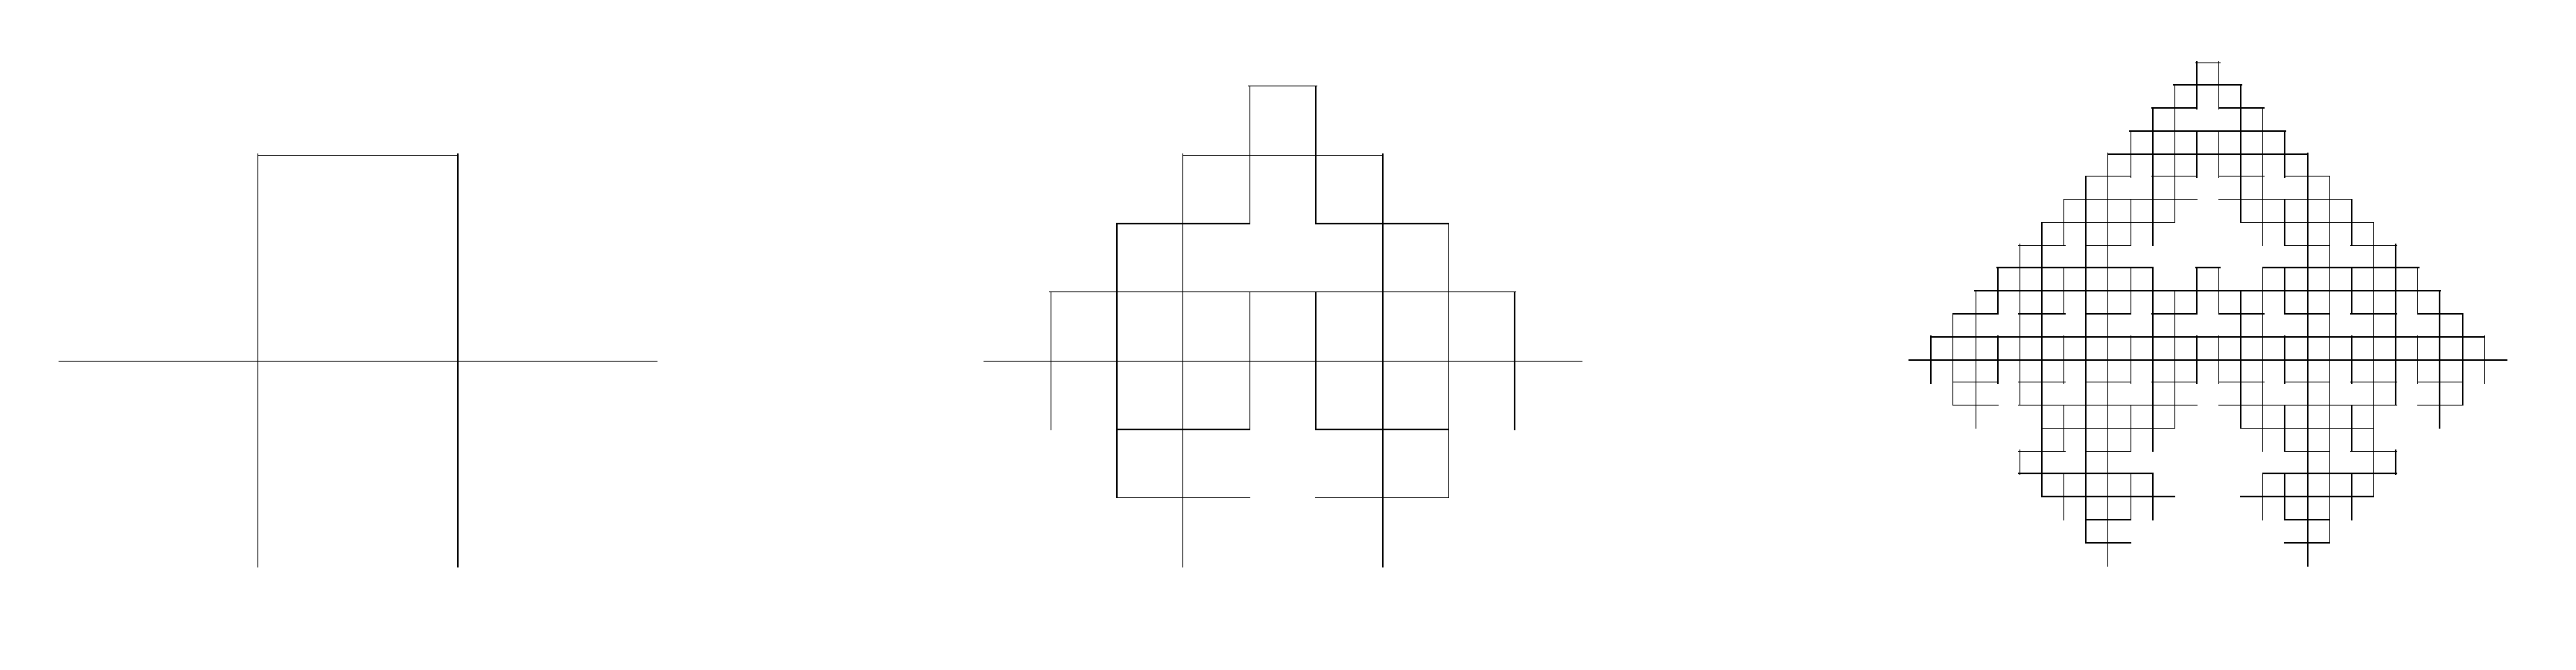
\includegraphics[width=6.0in]{Mandelbrot_Given}
   \caption[The Mandelbrot-Given curve with fractal dimension of $D_f=\ln_3 8$.]{The Mandelbrot-Given curve with fractal dimension of $D_f=\ln_3 8$.  The initial structure shown on the left is composed of eight line segments each with length $L=1/3$.  The higher orders of the fractal structure are generated by replacing each line segment with the initial structure.  Courtesy of K.M. Svensson.
}
\label{fig-mandelbrot}
\end{figure}
%


The dimension that was obtained using the coverage procedure just outlined is called the capacity dimension.  The definition of the dimension in terms of the capacity dimension is useful for the purpose of obtaining the corresponding dimension for a system with random distribution of measures, in particular, for multifractals.
To illustrate the concept of multifractality, we consider the critical eigenstate $|\Psi\rangle=\sum_{i=1}^{L^d}\psi_i|i\rangle$ of an electron at the metal to insulator transition.
Recall that $\vert i\rangle$ is a basis state at site $i$ with wavefunction amplitude $\psi_i$ and the eigenstate is a superposition of all the orthonormal basis states.  This wavefunction corresponds to a three-dimensional cubic lattice of linear length $L$ and volume $V=L^d$.  The wavefunction is normalized such that $\sum_{i=1}^{L^d}\psi_i=1$ and no site has exactly zero $\psi_i$.  This critical state possesses very interesting characteristics.  The values of the wavefunction amplitudes greatly fluctuate from site to site.  Even more, these large fluctuations in $\psi_i$ appear in all length scales, i.e., the fluctuations persist even when the scale at which the eigenstate is observed is varied.  There are points in the wavefunction containing large values of $\psi_i$ and the existence of sites having very small $\psi_i$ such that the distribution function of $\psi_i$ is broad. 
We apply the coverage procedure by dividing the system equally into smaller boxes.  One notices that different boxes enclose different substructures or densities.  The number of boxes enclosing one similar structure gives one fractal dimension.  In fact, a multitude of fractal dimensions is needed to completely characterize the full extent of the complex distribution that defines a system.  Systems of this kind are called multifractals because they are made up of different fractal sets.
This work probes the multifractal characteristics of the electronic eigenstate at the critical point and in the critical regime of the Anderson metal to insulator transition.




















%%%%%%%%%%%%%%%%%%%%%%%%%%%%%%%%%%%%%%%%%%%%%%%%%%%%%%%%%%%%%%%%%%%%%%%%%%
% $Log: MFA-theory.tex,v $
% Revision 1.7  2010/03/26 18:56:10  phrfar
% *** empty log message ***
%
% Revision 1.6  2010/03/24 16:12:00  phrfar
% edited, revised
%
% Revision 1.5  2010/03/11 19:37:10  phrfar
% *** empty log message ***
%
% Revision 1.4  2010/03/10 18:37:13  phrfar
% almost finished here
%
%%%%%%%%%%%%%%%%%%%%%%%%%%%%%%%%%%%%%%%%%%%%%%%%%%%%%%%%%%%%%%%%%%%%%%%%%%

%%%%%%%%%%%%%%%%%%%%%%%%%%%%%%%%%%%%%%%%%%%%%%%%%%%%%%%%%%%%%%%%%%%%%%%%%%
\chapter{Theory of Multifractal Analysis}
%%%%%%%%%%%%%%%%%%%%%%%%%%%%%%%%%%%%%%%%%%%%%%%%%%%%%%%%%%%%%%%%%%%%%%%%

%%%%%%%%%%%%%%%%%%%%%%%%%%%%%%%%%%%%%%%%%%%%%%%%%%%%%%%%%%%%%%%%%%%%%%%%
\section{Mass Exponents and Generalized Dimensions}
\label{sec-gIPR}
%%%%%%%%%%%%%%%%%%%%%%%%%%%%%%%%%%%%%%%%%%%%%%%%%%%%%%%%%%%%%%%%%%%%%%%%

We start by considering the distribution of the normalized wavefunction
intensities $\vert\psi\vert^2$ in the multifractal electronic state at the
critical point of the Anderson metal to insulator transition.  Using the usual
box counting method, we extract the multifractal properties of this
wavefunction.   Let  $\vert\psi_i\vert^2$ be the value of the wavefunction
intensity at the $i$-th site in a discretized $d$-dimensional system with volume
$L^d$.
If we cover the system equally with $N_l$ boxes each with linear size $l$, the
probability to find the electron in the $k$-th box is simply given by
%
\begin{equation}
	\mu_k(l)=\sum_{i=1}^{l^d} \vert\psi_i\vert^2,\quad k=1,\ldots,N_l.
	\label{eq-mudef}
\end{equation}
%
The box probability $\mu_k(l)$ constitutes the normalized measure
$\sum_{\mathrm{all~boxes}} \mu_k(l)=1$.
In the limit that $l\rightarrow 1$ (i.e., $l$ is equal to the lattice spacing),
the box probability reduces to the $\vert\psi_i\vert^2$.
The sum of the moments of the box probability over all boxes in the volume
%
\begin{equation}
 	P_q (l)=\sum_{k=1}^{N_l}\mu_k^q(l),
	\label{eq-IPRdef}
\end{equation}
%
is called the generalized inverse-participation ratios (gIPR).  The gIPR serve
as a $q$-microscope to effectively probe the fluctuations in
$\vert\psi_i\vert^2$.  The positive $q$ enhances the contribution coming from
the large $\vert\psi_i\vert^2$ while the negative $q$ is a region where the
small $\vert\psi_i\vert^2$ dominate.  For $q=2$, the gIPR is simply
the usual IPR $P_2=\sum_i \vert\psi_i\vert^4$ which is inversely proportional to the
number of sites contributing to a state.


The general assumption underlying multifractality is that within a certain range
of values for the ratio $\lambda\equiv l/L$, the moments
$P_q$ show a power-law behaviour indicating the absence of length scales in the
system,\cite{Jan94a}
%
\begin{equation}
	\label{eq-IPRscale}
	P_q (\lambda)\propto\lambda^{\tau(q)}.
\end{equation}
%
The exponent $\tau(q)$ is the mass exponent and is defined as
%
\begin{equation}
 	\tau(q)=\lim_{\lambda\rightarrow0}
\frac{\mathrm{log}~P_q(\lambda)}{\mathrm{log}~\lambda},
\end{equation}
where the limits states that the true value of $\tau(q)$ at
criticality is in the thermodynamic limit $\lambda\rightarrow0$.
The values for $\tau(q)$ in the limiting cases of weak and strong disorder and
at the MIT are
%
\begin{equation}
	\tau(q) = 
	\begin{array}{ll}
	d (q-1) & \textrm{for metals,}\\
	0 & \textrm{for insulators }(q>0),\\
	D_q (q-1) & \textrm{at the MIT}.
	\end{array}
\end{equation}
%
In an extended metallic state where the wavefunction intensity is uniformly
distributed as $\vert\psi_i\vert^2\propto L^{-d}$ and $d$ is the dimension of
the support, $P_q$ is a linear function of $q$ with slope $d=3$ for a $3D$
system.  For a strong disorder state where the wavefunction is highly localized
within one small spatial region, $P_q=1$ for all positive $q$'s and hence $\tau=0$.  An
indication that a state is multifractal is when $\tau(q)$ is a nonlinear
function of $q$.  Generally, $\tau(q)$ is a non-decreasing convex function.
At criticality, $\tau(q)$ can also be parametrized as
$\tau(q)=d(q-1)+\Delta_q$, where $\Delta_q$ are the anomalous scaling exponents
characterizing the critical point \cite{EveMM08}.  Furthermore, from
Eqs.~\eqref{eq-IPRdef} and \eqref{eq-IPRscale} it is easy to see that $\tau(0)=-d$
and due to the normalization condition $\tau(1)=0$.


The values of $\tau(q)$ will give the set of generalized dimensions $D_q$ that
defines the multifractal system.  To show that this is the case, we consider for
the present purpose a uniform distribution of $\vert\psi_i\vert^2$ on a support
with fractal dimension $D_f$.  Using the normalization condition, we can say
that the box probability can be expressed as $\mu_k(l)\propto l^{D_f}L^{-D_f}$
since $\vert\psi_i\vert^2\propto L^{-D_f}$ and the number of sites in a box is
proportional to $l^{D_f}$.
Take note that the assumption of normal distribution for $\vert\psi\vert^2$
allows the relation $\vert\psi_i\vert^2\propto L^{-D_f}$ to be valid for all $q$
and that $D_f$ to be independent of $q$.  The gIPR can then be reformulated as
%
\begin{equation}
	\label{eq-IPRDq}
 	P_q(\lambda)\propto\lambda^{D_f(q-1)},
\end{equation}
%
where the summation in Eq.~\eqref{eq-IPRdef} is replaced by the number of boxes
$N_l=(\frac{L}{l})^{D_f}$.
Comparing equations \eqref{eq-IPRscale} and \eqref{eq-IPRDq}, we can see that
$\tau(q)=D_f (q-1)$.  If the distribution of the measure is not normal such that
the fractal dimension depends on $q$ then $\tau(q)=D_q (q-1)$.  The set of
generalized fractal dimensions is then given as
%
\begin{equation}
 D_q=\frac{1}{q-1}\lim_{\lambda\rightarrow0}\frac{\mathrm{log}~P_q(\lambda)}{
\mathrm{log}~\lambda}. \end{equation}
%
$D_q$ is a monotonically decreasing positive function of $q$
As with $\tau(q)$, the $q$-dependence of $D_q$ is an indication of multifractality.
The physical meaning of some of the dimensions will be given here.  For $q=0$,
$D_0$ is equal to the dimension of the support of the measure.  $D_1$ is
equivalent to the information dimension of the system which is in statistical
mechanics related to the entropy of the probability distribution of box
probabilities $S_\lambda=-\sum_{N_l}\mu_k(\lambda)\mathrm{log}\mu_k(\lambda)$. 
The generalized dimension corresponding to $q=2$ is related to the correlation
dimension that for a system partitioned into boxes gives the probability that the distance between two points in the state is
less than the box size.


%%%%%%%%%%%%%%%%%%%%%%%%%%%%%%%%%%%%%%%%%%%%%%%%%%%%%%%%%%%%%%%%%%%%%%%%
\section{Relation between the Mass Exponents and Singularity Spectrum}
\label{sec-tau&falph}
%%%%%%%%%%%%%%%%%%%%%%%%%%%%%%%%%%%%%%%%%%%%%%%%%%%%%%%%%%%%%%%%%%%%%%%%
%%%%%  meaning of "scales as "

We shall demonstrate that the mass exponents $\tau(q)$ are related to a set of fractal dimensions
called the singularity spectrum $f(\alpha)$ and that they
are exactly equivalent such that a multifractal state is completely
defined by either one of them.
Again, we consider the multifractal distribution of the wavefunction intensities
with volume $L^d$ and we divide it into boxes of length $l$.  If we take one box
probability $\mu_1$, we will find that its value will have a $\lambda$ dependence as
$\mu_1(\lambda)\sim\lambda^{\alpha_1}$ to some exponent $\alpha_1$.  Another
box would scale to another exponent as $\mu_2(\lambda)\sim\lambda^{\alpha_2}$.  In fact, different boxes scale
to different exponents $\alpha$.  Furthermore, the number of these boxes, $N_{\alpha'}$, corresponding to
the same $\alpha=\alpha'$ scales as $N_{\alpha'}\propto\lambda^{-f(\alpha')}$.  The set of boxes that scale to the same $\alpha=\alpha'$ is a fractal with a fractal dimension of $f(\alpha')$.  A multifractal state such as the electronic state at the MIT is completely defined by a an infinite set of $f(\alpha)$ values which is called the singularity spectrum.

The ensemble (arithmetic) average of the generalized inverse participation ratios in terms of the probability density function (PDF) of the box probability $\mathcal{P}(\mu_k)$ is given by
%
\begin{equation}
\label{eq-IPRasPDF1}
 \lambda^{-d}\langle\mu_k^q(\lambda)\rangle=\lambda^{-d}\int_0^1 \mathcal{P}(\mu_k)~\mu_k^q(\lambda)~\ud \mu_k,
\end{equation}
%
where the average is over all disorder realizations and over the lattice volume $L^d$.  The normalization of $\mu_k(\lambda)$ gives the limits of the integration. 
We make a change of variables, $\mathcal{P}(\mu_k)\ud\mu_k=\mathcal{P}(\alpha)\ud\alpha$.  In terms of $\alpha$, we parametrize the box probability to be $\mu_k(\lambda)\equiv \lambda^\alpha$ and its logarithmic form is $\alpha\equiv\ln\mu_k/\ln\lambda$.  When $l=1$, the box probability reduces to the wavefunction intensity that is given by $\vert\psi_i\vert^2\equiv L^{-\alpha}$.
Furthermore, $\mu_k^q(\lambda)=\lambda^{\ln_\lambda \mu_k^q}=\lambda^{q\frac{\ln\mu_k}{\ln\lambda}}$.  Equation \eqref{eq-IPRasPDF1} becomes
%
\begin{equation}
\label{eq-IPRasPDF2}
 \lambda^{-d}\langle\mu_k^q(\lambda)\rangle=\lambda^{-d}\int_0^\infty \mathcal{P}(\alpha)~\lambda^{q\alpha}~\ud\alpha.
\end{equation}
%
In terms of the PDF $\mathcal{P}(\alpha)$, the number of boxes having the same values of $\mu_k=\lambda^\alpha$ is $N_\alpha=\mathcal{P}(\alpha)\ud\alpha\cdot \lambda^{-d}\propto \lambda^{-f(\alpha)}$.  Hence, using $\mathcal{P}(\alpha)\propto \lambda^{d-f(\alpha)}$ into Eq.~\eqref{eq-IPRasPDF2} we have
%
\begin{eqnarray}
\label{eq-IPRasPDF3}
 \lambda^{-d}\langle\mu_k^q(\lambda)\rangle & \propto & \int_0^\infty \lambda^{q\alpha-f(\alpha)}~\ud\alpha \nonumber\\
					    & \propto & \int_0^\infty e^{\ln\lambda\cdot \tilde{F}(\alpha)}~\ud\alpha,
\end{eqnarray}
%
where $\tilde{F}(\alpha)=q\alpha-f(\alpha)$.  We evaluate the above integral using the saddle-point method which is justified in the limit of large $L$ or small $\lambda$.  The saddle-point method requires that the function $\tilde{F}(\alpha)$ must have a unique global maximum at some $\alpha=\tilde{\alpha}$, i.e, $\tilde{F}''(\tilde{\alpha})<0$, and that $\tilde{\alpha}$ is not an end point in the integration interval.  
Solving the integral of Eq.~\eqref{eq-IPRasPDF3} reproduces the scaling relation in \eqref{eq-IPRscale} and gives the following relations
%
%
\begin{equation}
\label{eq-qdef}
 q=f'(\tilde{\alpha}),
\end{equation}
%
\begin{equation}
 \label{eq-falphadef}
 \tau(q)=q\tilde{\alpha}-f(\tilde{\alpha}),\qquad 
 f(\tilde{\alpha})=q\tilde{\alpha}-\tau(q).
\end{equation}
%
Furthermore using Eq.~\eqref{eq-falphadef} into Eq.~\eqref{eq-qdef}, we will obtain
%
\begin{equation}
 q=q+\tilde{\alpha}\frac{\ud q}{\ud\alpha}-\frac{\ud\tau}{\ud q}\frac{\ud q}{\ud\alpha},
\end{equation}
which gives the values of the singularity strength or the Lipschitz-H$\ddot{o}$lder exponent to be
%
\begin{equation}
 \label{eq-alphadef}
 \tilde{\alpha}_q=\frac{\ud\tau(q)}{\ud q}.
\end{equation}
%
Equations \eqref{eq-qdef} to \eqref{eq-alphadef} state that $f(\alpha)$ is just the Legendre transformation of $\tau(q)$.
Furthermore, since $q=f'(\tilde{\alpha})$ then the maximum of the singularity spectrum can exactly be found at $q=0$.


The singularity spectrum $f(\alpha)$ is a convex function of $\alpha$.  
A pictorial sketch of the properties of $f(\alpha)$ is shown in Fig.~\ref{fig-sexyfalfa}.
%
\begin{figure}
 	\includegraphics[width=\figwidth]{fig-sexyfalfa.eps}
	\caption[Pictorial representation of the general features of the multifractal spectrum at criticality.]{Pictorial representation of the general features of the multifractal spectrum at criticality. The dotted purple areas highlight forbidden regions for $f(\alpha)$.
		Each point on the spectrum corresponds exactly to an evaluation of a $q$-moment of the gIPR.
		The maximum is found at the point $q=0$ where $f(\alpha_0)=d$.  At $q=1$, $f(\alpha_1)=\alpha_1$ and $f'(\alpha_1)=1$.
		The two regions to the right and left of $q=1/2$ are determined by different  wavefunction amplitudes, $|\psi_i|^2 > L^{-d}$ (white) and $|\psi_i|^2<L^{-d}$ (yellow).
                The symmetry axis at $q=1/2$ is highlighted and here $f(\alpha_{1/2}=d)=d-\Delta_{1/2}$.
		The yellow shaded area can be connected to the white area via the symmetry relation \eqref{eq-symalfaq},\eqref{eq-symfalfa}, and vice versa.
		The points corresponding to $q=0$ and $q=1$ are symmetry related points.}
	\label{fig-sexyfalfa}
\end{figure}
%
Due to the normalization condition of $\vert\psi_i\vert^2$, $f(\alpha)$ is only defined on a semi-axis $\alpha\geq0$.  It has its maximum at $\alpha_0 \geqslant d$ where $f(\alpha_0)=d$.  Since nowhere in the wavefunction will $\vert\psi_i\vert^2=0$, $d$ is simply the topological dimension.  As previously shown, $\alpha_0$ corresponds exactly to the moment $q=0$ evaluation of the gIPR.  To the right of $\alpha_0$ is the region of negative $q$'s where the contributions coming from small wavefunction intensities $\vert\psi_i\vert^2<L^{-d}$ are dominant.  The left region at $\alpha<\alpha_0$ of the singularity spectrum is the positive $q$'s area that is being populated by large $\vert\psi_i\vert^2>L^{-d}$.
For $\alpha_1$ that corresponds to $\tau(1)=0$, we have $f(\alpha_1)=\alpha_1$ and $f^\prime (\alpha_1)=1$. 
In the limit of vanishing disorder the singularity spectrum becomes narrower and
eventually converges to one point $f(d)=d$. On the other hand, as the value of
disorder increases the singularity spectrum broadens and
in the limit of strong localisation the singularity spectrum tends to converge
to the points:  $f(0)=0$ and $f(\infty)=d$.
Only at the MIT we can have a true multifractal behaviour and as a consequence
the singularity spectrum must be independent of all length scales, such as
the system size.
%% insert f(alpha) figures

%%%%%%%%%%%%%%%%%%%%%%%%%%%%%%%%%%%%%%%%%%%%%%%%%%%%%%%%%%%%%%%%%%%%%%%%
\section{Parabolic Approximations to the $f(\alpha)$}
\label{sec-parabola}
%%%%%%%%%%%%%%%%%%%%%%%%%%%%%%%%%%%%%%%%%%%%%%%%%%%%%%%%%%%%%%%%%%%%%%%%

From an analytical viewpoint not much is known about how the singularity spectrum should look like at criticality.  However, an approximate expression for the $f(\alpha)$ has been put forward that is valid in the regime of weak multifractality, i.e.\ when the critical point is close to a metallic behaviour.
This applies to the Anderson transition in $d=2+\epsilon$ dimensions with $\epsilon \ll 1$. In this case a parabolic dependence of the singularity spectrum is found to be \cite{Weg89}
%
\begin{equation}
 f(\alpha) \simeq d-\frac{\left[\alpha -(d+\epsilon)\right]^2}{4\epsilon}.
 \label{eq-parabola}
\end{equation}
%
Equation \eqref{eq-parabola} implies a corresponding approximation for the anomalous dimensions as given by $\Delta_q\simeq -\epsilon q(q-1)$. 
For the case of $d=2+1$, we have $f(\alpha)=d-(\alpha-\alpha_0)^2/4$.
This parabolic approximation for the $f(\alpha)$, apart from the dimension of the support $d$, only depends on one parameter $\alpha_0$ that is exactly $\alpha_0=4$ for $d=2+1$ case and that defines the position of the maximum $f(\alpha_0)=d$.  Generally, equation \eqref{eq-parabola} provides a very good approximation to the critical $f(\alpha)$ near $\alpha=\alpha_0$ and deviates from the true $f(\alpha)$ at $\alpha$ values far away from $\alpha_0$.
Due to the normalization condition of the wavefunction intensities, we have to impose the condition $\alpha\geqslant0$ to Eq.~\eqref{eq-parabola}.  In the limit of $\alpha=0$ such that $\alpha=\frac{\ud\tau(q)}{\ud q}=0$, the mass exponent $\tau(q)$ should approach a constant value as $q\rightarrow q_c$ where critical $q_c$ corresponds to $\alpha_{q_c}=0$.
Therefore, the parabolic $f(\alpha)$ should terminate at $\alpha=0$ with a finite value.  This behaviour is known as the termination of the multifractal spectrum.
%However, the exact parabolicity fails in the limit of $q\rightarrow\infty$ when $q=f'(\alpha)=\infty$.  That is when $f(\alpha)$ approaches $\alpha=0$ with an infinite slope and $f(\alpha=0)=-\infty$.  This scenario is equivalent to the situation when $\tau(q)$ continues to increase for $q\rightarrow\infty$.
Whether the $f(\alpha)$ at $\alpha=0$ terminates or continues to negative infinity will be further discussed later on.
Although the parabolic approximation has turned out to be exact for some models \cite{LudFSG94} its validity, in particular  for the integer quantum Hall transition, is currently under an intense debate \cite{ObuSFGL08} due to the implications that this result has upon the critical theories describing the transition.

%%%%%%%%%%%%%%%%%%%%%%%%%%%%%%%%%%%%%%%%%%%%%%%%%%%%%%%%%%%%%%%%%%%%%%%%
\section{Symmetry Relations in the Multifractal Spectrum at the Anderson Transition}
\label{sec-symmetry}
%%%%%%%%%%%%%%%%%%%%%%%%%%%%%%%%%%%%%%%%%%%%%%%%%%%%%%%%%%%%%%%%%%%%%%%%

Recently, the existence of exact symmetry relations in the multifractal exponents of the Anderson transition has been reported \cite{MirFME06}.
The mass exponents that describe the scaling of the generalized inverse participation ratio in Eq.~\eqref{eq-IPRscale} can be defined at criticality to be $\tau(q)=d(q-1)+\Delta q$.
The anomalous exponents $\Delta_q$ separate the critical point from the metallic phase for which $\Delta_q=0$.
Furthermore, $\Delta_q$ determine the scale dependence of the moments of the local density of states (LDOS) $\rho^q$ \cite{EveMM08} that is expressed as 
%
\begin{equation}
\label{eq-LDOSscale}
\langle\rho^q\rangle\propto L^{-\Delta_q}. 
\end{equation}
%
Previous works have suggested a symmetry relation in the distribution function of LDOS $\mathcal{P}_\rho(\tilde{\rho})$ as given by
%
\begin{equation}
 \label{eq-symPDFLDOS}
 \mathcal{P}_\rho(\tilde{\rho})=\tilde{\rho}^{-3}\mathcal{P}_\rho(\tilde{\rho}^{-1}),
\end{equation}
%
where $\tilde{\rho}=\rho/\langle\rho\rangle$ is the normalized LDOS.
Since $\langle\tilde{\rho}^q\rangle=\int \ud\tilde{\rho}~\tilde{\rho}^q~\mathcal{P}_\rho(\tilde{\rho})$, Eq.~\eqref{eq-symPDFLDOS} implies the relation $\langle\tilde{\rho}^q\rangle=\langle\tilde{\rho}^{1-q}\rangle$ which from Eq.~\eqref{eq-LDOSscale} in turn gives
%
\begin{equation}
\label{eq-symDeltaq}
 \Delta_q = \Delta_{1-q}.
\end{equation}
%
Equation \eqref{eq-symPDFLDOS} has been derived using a supersymmetric nonlinear $\sigma$ model \cite{MirF94} that is able to approximately model the critical properties of the Anderson transition for the case of weak disorder but breaks down for strong disorder.
It has been argued that although the mapping of the Anderson model onto the nonlinear $\sigma$ model is not exact, there exist several microscopic models (e.g., $N$-orbital Wegner model for $N\rightarrow\infty$) for the Anderson transition that can be reduced exactly to the nonlinear $\sigma$ model.  The universality of the critical exponents permits the validity of the symmetry relation \eqref{eq-symDeltaq} in the multifractal exponent $\Delta_q$ on any microscopic model of criticality.

In terms of the mass exponents and $\tau(1-q)=d(1-q-1)+\Delta_{1-q}$, Eq.~\eqref{eq-symDeltaq} can also be written as
%
\begin{equation}
\label{eq-symTauq}
 \tau(q)-\tau(1-q)=d(2q-1).
\end{equation}
%
Equations \eqref{eq-symDeltaq} and \eqref{eq-symTauq} reveal the existence of the symmmetry axis at $q=1/2$.
Furthermore, expressing $\tau(q)$ in its Legendre transform of $f(\alpha_q=\frac{\ud\tau_q}{\ud q})$ and since $-\alpha_{1-q}=\frac{\ud\tau_{1-q}}{\ud (1-q)}\frac{\ud (1-q)}{\ud q}$, the corresposponding symmetry relations are given by
%
\begin{equation}
 	\alpha_q + \alpha_{1-q} = 2d,
	\label{eq-symalfaq}
\end{equation}
%
\begin{equation}
 	f(2d-\alpha) = f(\alpha) +d -\alpha.
	\label{eq-symfalfa}
\end{equation}
%
Equation \eqref{eq-symfalfa} follows from using the relations \eqref{eq-symTauq} and \eqref{eq-symalfaq} into the definition of $f(\alpha_{1-q})=(1-q)\alpha_{1-q}-\tau_{1-q}$.  In Fig.~\ref{fig-sexyfalfa}, we highlight the symmetry points and relations in the critical multifractal spectrum.


We shall look at the implications of these symmetry relations on the multifractal spectrum.
%
%
%  DISCUSS  !!!!!!!!!!!!!
%  situations where symmetry is not valid nor satisfied
%  termination points, freezing
% slope of f(alpha) at q-> infntt  at the TAILS depending on typical or ensemble
%
%
The wave function normalization condition gives the lower bound $\alpha_{\mathrm{min}}=0$ for the singularity strength and requires that $\alpha$ is always positive.
It readily follows from the symmetry in \eqref{eq-symalfaq} that in the limit of $\alpha_{q\rightarrow+\infty}$ then $\alpha_{q\rightarrow+\infty}+\alpha_{q\rightarrow-\infty}=2d$ which means that $\alpha$ should only be contained in the interval $[0,2d]$.  If $\alpha_{q\rightarrow+\infty}=0$ then the upper bound is $\alpha\leqslant 2d$.
%
Furthermore, the symmetry relation in the singularity spectrum $f(\alpha)$ states that $0\leqslant \alpha \leqslant d$ and $d\leqslant \alpha \leqslant
2d$ regions of the singularity spectrum must be related by the relation \eqref{eq-symfalfa}.  In other words, using \eqref{eq-symfalfa} one can be mapped onto another.  The symmetry axis $\alpha=d$ is exactly equivalent to $q=\frac{1}{2}$.


Numerical calculations have since then supported this symmetry in  $f(\alpha)$ in the one-dimensional power-law random-banded-matrix model \cite{MirFME06} and the two-dimensional Anderson transition in the spin-orbit symmetry class \cite{ObuSFGL07} and SU2 model \cite{MilE07}.  In the present work we numerically verify that this symmetry in the singularity spectrum also holds in the three-dimensional (3D) Anderson model. In order to address this hypothesis with sufficient accuracy, we have considered the box- and system-size scaling of the typical and ensemble averages of $P_q$ in computing the $f(\alpha)$. We discuss which numerical strategy will produce the best possible agreement with the symmetry and we highlight the statistical analysis that must be used to observe the reported symmetries with sufficient confidence.
%%%%%%%%%%
%
%
% DISCUSS
% benefits of symmetry
% symmetry found to be true in critical acoustic waves, french guys, other non-Anderson analytical model
%


%\include{MFA-typ}
%\include{MFA-ens}
%\include{MFA-partitioning}
%\include{MFA-PDF}
%\include{FSS}

%%%%%%%%%%%%%%%%%%%%%%%%%%%%%%%%%%%%%%%%%%%%%%%%%%%%%%%%%%%%%%%%%%%%%%%%%%
\chapter{Conclusion}
%%%%%%%%%%%%%%%%%%%%%%%%%%%%%%%%%%%%%%%%%%%%%%%%%%%%%%%%%%%%%%%%%%%%%%%%%%

As a summary this work has made a careful and systematic study on the multifractal characteristics at the critical point and in the critical regime of the electronic state within the Anderson model of localisation using high-precision data and very large system sizes.  It has demonstrated that the best strategy to obtain a complete picture of the multifractal spectrum, which contains negative fractal dimensions and shows the contributions coming from the tails of the distribution, and to find better agreement with the proposed symmetry in the multifractal exponents is to use system-size scaling with ensemble averaging in which to specifically consider a sensible range of system sizes with very large number of states.
From the multifractal analysis, we extract information about critical properties of the Anderson transition such as the following: validity of the symmetry relation in the multifractal exponents and probability distribution function (PDF) of wavefunction intensities, existence of rare events which give rise to negative fractal dimensions, critical disorder and critical exponent which describes the divergence of the correlation length near the critical point.  The multifractal analysis has also allowed us to comment and give speculations about the non-parabolicity of the multifractal spectrum, non-Gaussian nature of the PDF and possibility of termination points in the $f(\alpha)$.  Lastly, this work has proposed an alternative method that is numerically simpler to obtain the multifractal spectrum from the PDF of wavefunction intensities.

In the following, we highlight the important results of this work.

\begin{enumerate}

\item 
Using state of the art diagonalization technique for sparse matrices, we have reached very large system sizes of up to 		
$L^3=240^3$ which corresponds to wavefunction sites of $1.4\times 10^7$.  The statistics involved in this work is unprecedented.  
At the approximated critical point, we have used $\sim 5\times 10^4$ states for $L\leqslant100$ and $\sim 100$ states for $L> 100$.  
In the critical regime corresponding to disorder values from $15.0$ to $18.0$, we have taken at least $10000$ uncorrelated samples for each size $L\in [20,30,\cdots,100]$ and disorder combination, for a total of $1,530,000$ wave functions.
%
The huge statistics involved here have allowed us to reach regimes such as the tails of the multifractal spectrum that are highly sensitive to finite size effects and number of disorder realizations.

\item
The study has given an in-depth analysis on the role of different averaging and the effect of system- and box- size scaling to the shape of the critical multifractal spectrum.  The latter scaling approach is necessary to estimate the behaviour in the thermodynamic limit that is being reached faster by using system-size scaling which by varying $L$ considers different disorder realizations and reduces finite size effects.
%
In using a typical average which is dominated by a single representative site, an increase of disorder realization will only change the $f(\alpha)$ shape up to a point but increasing $L$ will cause the $f(\alpha)$ to shift towards the left, i.e., lower values of $\alpha^{typ}$ and $f^{typ}$.
%
On the other hand, the $f^{ens}(\alpha)$ obtained from the use of ensemble average which considers contributions from all disorder realizations equally is shown to be dependent on the number of disorder realizations.  Furthermore, it gives a complete profile of the spectrum because it contains information about negative fractal dimensions which is lost with typical averaging.  The study has demonstrated that for a fixed $L$,
$f^{ens}(\alpha)$ reaches more negative values upon an increase in disorder realizations.  Since the regions of the negative fractal dimension is caused by the so-called rare events of whose number decreases with $L$, an increase in $L$ must be accompanied with an increase in the disorder realizations to see the same extent of negative fractal dimensions.

\item
This work has demonstrated the validity of a proposed symmetry relation in the multifractal exponents in the 3D Anderson Model within the orthogonal universality class.  The statistical analysis have shown that the symmetry relation is true in the thermodynamic limit since better agreement to the symmetry relation is satisfied whenever higher number of disorder realizations and larger system sizes are considered.  
Better agreement to the symmetry is found whenever the $f(\alpha)$ reaches more negative values, $\alpha$ moves closer to zero and the right $f(\alpha)$ satisfies the upper limit of $\alpha\leq 2d$
The best strategy to satisfy the symmetry to use system-size scaling with ensemble averaging in which to specifically consider a sensible range of system sizes with very large number of states.

\item
In pursuit of a numerical optimisation of the box-scaling technique we discuss  different box-partitioning schemes including cubic and non-cubic boxes, use of periodic boundary conditions to enlarge the system and single and multiple origins  for the partitioning grid are also implemented.  We show that the numerically most reliable method is to divide a system of linear size $L$ equally into cubic boxes of size $l$ for which $L/l$ is an integer. This method is the least numerically expensive while having a good reliability.



\end{enumerate}




















%  \appendix                            %% this will do the appendices
%  \chapter{Proof of Fred's theorem}
%  \input{app1.tex}
%  \chapter{listing of Fred's program}
%  \input{app2.tex}
\begin{singlespace}
\bibliographystyle{unsrt}
\bibliography{bibliograph}            %% Start your bibliography here; 
\end{singlespace}

                                 %! with sample.bib as your bibliography file. You can
                               %% also use:
                %! \begin{thebibliography}
                %!    \bibitem{etc....
                %! \end{thebibliography}
                               %% to generate your bibliography.

%\begin{thesisauthorvita}             %% Write your vita here; it can be
%                                     %% anything in LaTeX2e par-mode.
%\end{thesisauthorvita}               %%


\end{document}                       %% Done.
